
\documentclass[10pt,journal,compsoc]{IEEEtran}

\IEEEoverridecommandlockouts
\usepackage{graphicx}

\ifCLASSOPTIONcompsoc
    \usepackage[caption=false, font=normalsize, labelfont=sf, textfont=sf]{subfig}
\else
\usepackage[caption=false, font=footnotesize]{subfig}
\fi

\usepackage{graphicx}
\usepackage{cite}
\usepackage{amsfonts}
\usepackage{amsmath}
\usepackage{amsxtra}
\usepackage{amsbsy}
\usepackage{floatflt}
\usepackage{amssymb}
\usepackage{tabularx}
\usepackage{multirow}
\usepackage{nth}
\usepackage{comment}
\usepackage{epstopdf}
\usepackage{hhline}
\usepackage{siunitx}
\usepackage{booktabs}
\usepackage[bottom]{footmisc}
\usepackage[acronym]{glossaries}
\glsdisablehyper
\usepackage{upgreek}
\usepackage{algorithm}
\usepackage{algorithmicx,algpseudocode}
\usepackage{algpseudocode}
\usepackage{bm}
\usepackage[utf8]{inputenc}
\usepackage{lipsum}
\usepackage{array} 
\usepackage{epsfig}
\usepackage{times}
\usepackage{framed}
\usepackage{enumitem}
\usepackage{float}
\usepackage{etoolbox}
\usepackage{lipsum}
\usepackage{soul}
\usepackage{mathtools}
\usepackage{bbm}
\usepackage{makecell}
\usepackage{pifont}
\usepackage[export]{adjustbox} 
\usepackage{latexsym}
\usepackage{multicol}
\usepackage{eurosym}
\usepackage{xspace}
\usepackage{pdfpages}
\usepackage{verbatim}
\usepackage{stfloats}
\usepackage{blindtext}
\usepackage{colortbl}
\usepackage{xfrac}
\usepackage{relsize}


\newtheorem{problem}{Problem}

\newcommand{\tbd}[1]{{\color{red}{[TBD] #1}}}
\newcommand{\rmmult}{\scriptscriptstyle\mathrm{mult}}
\newcommand{\ssub}[1]{{\scriptscriptstyle { #1}}}
\newcommand{\change}[1]{{\color{blue} {#1}}}
\newcommand{\addcomment}[1]{{\textcolor{red}{\hl{\em$[$#1$]$}}}}
\newcommand{\rmref}{\scriptscriptstyle\mathrm{ref}}
\newcommand{\name}{COLoRIS}

\newcommand{\mb}[1]{\mathbf{{#1}}}
\newcommand{\tran}{\mathrm{T}}
\newcommand{\herm}{\mathrm{H}}
\newcommand{\diag}{\mathrm{diag}}
\newcommand{\tr}{\mathrm{tr}}
\DeclareMathOperator{\erf}{erf}
\DeclareMathOperator{\cosine}{c}
\DeclareMathOperator{\sine}{s}

\newcommand{\floor}[1]{\lfloor #1 \rfloor}

\setlength{\textfloatsep}{3pt}
\setlength{\skip\footins}{8.2pt}


\newcommand{\fd}[1]{\textcolor{teal}{#1}}

\newcommand{\FD}[1]{\textcolor{teal}{\footnotesize \textsf{[Francesco: #1]}}}
\newcommand{\GE}[1]{\textcolor{purple}{\footnotesize \textsf{[Guillermo: #1]}}}

\newcommand\blfootnote[1]{
  \begingroup
  \renewcommand\thefootnote{}\footnote{#1}
  \addtocounter{footnote}{-1}
  \endgroup
}


%%%%%%%%% List of acronyms %%%%%%%%%%%

\newacronym{3d}{3D}{Three Dimensional}
\newacronym{ue}{UE}{User Equipment}
\newacronym[plural=RISs, firstplural=Reconfigurable Intelligent Surfaces (RISs)]{ris}{RIS}{Reconfigurable Intelligent Surface}
\newacronym{bs}{BS}{Base Station}
\newacronym{mimo}{MIMO}{Multiple-Input Multiple-Output}
\newacronym{miso}{MISO}{Multiple-Input Single-Output}
\newacronym{siso}{SISO}{Single-Input Single-Output}
\newacronym{upa}{UPA}{Uniform Planar Array}
\newacronym{ula}{ULA}{Uniform Linear Array}
\newacronym{aoa}{AoA}{Angle of Arrival}
\newacronym{aod}{AoD}{Angle of Departure}
\newacronym{snr}{SNR}{Signal to Noise Ratio}
\newacronym{kpi}{KPI}{Key Performance Indicator}
\newacronym{pdf}{PDF}{Probability Density Function}
\newacronym{pmf}{PMF}{Probability Mass Function}
\newacronym{fi}{FI}{Fisher Information}
\newacronym{crb}{CRB}{Cramér–Rao Bound}
\newacronym{csi}{CSI}{Channel State Information}
\newacronym{rv}{RV}{Random Variable}
\newacronym{pgm}{PGM}{Projected Gradient Method}
\newacronym{mse}{MSE}{Mean Squared Error}
\newacronym{ml}{ML}{Machine Learning}
\newacronym{mcu}{MCU}{Micro Controller Unit}
\newacronym{dnn}{DNN}{Deep Neural Network}
\newacronym{nlos}{NLoS}{non-Line of Sight}
\newacronym{los}{LoS}{Line of Sight}
\newacronym{soa}{SoA}{State-of-Art}
\newacronym{usart}{USART}{Universal Synchronous/Asynchronous Receiver/Transmitter}
\newacronym{usb}{USB}{Universal Serial Bus}
\newacronym{isac}{ISAC}{Integrated Sensing and Communication}
\newacronym{nn}{NN}{Neural Network}
\newacronym{slam}{SLAM}{Simultaneous Localization and Mapping}
\newacronym{iqr}{IQR}{Interquartile Range}


\begin{document}

\title{\name{}: Localization-agnostic Smart Surfaces Enabling Opportunistic ISAC in 6G Networks}

This work has been submitted to the IEEE for possible publication. Copyright may be transferred without notice, after which this version may no longer be accessible.


\author{Guillermo Encinas-Lago,~\IEEEmembership{Student Member,~IEEE,}
Francesco Devoti,~\IEEEmembership{Member,~IEEE,} \\
Marco Rossanese,~\IEEEmembership{Student Member,~IEEE,}
Vincenzo~Sciancalepore,~\IEEEmembership{Senior Member,~IEEE,}\\
Marco Di Renzo,~\IEEEmembership{Fellow,~IEEE,}
Xavier~Costa-P\'erez,~\IEEEmembership{Senior Member,~IEEE,}

\thanks{\textit{Guillermo Encinas-Lago is with NEC Laboratories Europe, 69115 Heidelberg, Germany and Universit\'e Paris-Saclay, CNRS, CentraleSup\'elec, Laboratoire des Signaux et Syst\`emes, 91190 Gif-sur-Yvette, France. 
Francesco Devoti, Marco Rossanese and Vincenzo Sciancalepore are with NEC Laboratories Europe. 
Marco Di Renzo is with Universit\'e Paris-Saclay, CNRS, CentraleSup\'elec, Laboratoire des Signaux et Syst\`emes. 
Xavier Costa-P\'erez is with i2cat, ICREA, 08034 Barcelona, Spain and NEC Laboratories Europe.
This work was supported by the EU SNS JU INSTINCT project under grant agreement no. 101139161.\newline
Email of the corresponding author: Guillermo.Encinas@neclab.eu.}}
}


\maketitle


\begin{abstract}
The integration of Smart Surfaces in 6G communication networks, also dubbed as \glsunset{ris}\acrlongpl{ris} (\glspl{ris}), is a promising paradigm change gaining significant attention given its disruptive features.
~\glspl{ris} are a key enabler in the realm of 6G \gls{isac} systems where novel services can be offered together with the future mobile networks communication capabilities.
This paper addresses the critical challenge of precisely localizing users within a communication network by leveraging the controlled-reflective properties of \gls{ris} elements 
without relying on more power-hungry traditional methods, e.g., GPS, adverting the need of deploying additional infrastructure and even avoiding interfering with communication efforts.
~Moreover, we go one step beyond: we build \name{}, an \emph{Opportunistic ISAC} approach that leverages localization-agnostic \gls{ris} configurations to accurately position mobile users via trained learning models. 
Extensive experimental validation and simulations in large-scale synthetic scenarios show $\textbf{5\%}$ positioning errors (with respect to field size) under different conditions.
Further, we show that a low-complexity version running in a limited off-the-shelf (embedded, low-power) system achieves positioning errors in the $\textbf{11\%}$ range  at a negligible $\textbf{+2\%}$ energy expense with respect to the classical \gls{ris}. 
\end{abstract}

\begin{IEEEkeywords}
Localization, Reconfigurable intelligent surfaces, Deep learning, Integrated sensing and communication
\end{IEEEkeywords}



\glsresetall

\section{Introduction}
\label{sec:introduction}

In the ever-evolving landscape of modern technology, the implementation of emerging technology, such as \glspl{ris},\footnote{Note that the terms \gls{ris} and Smart Surface can be used interchangeably within the paper, as they refer to the same physical device.} has emerged as a transformative force, reshaping the way we perceive and interact with the propagation environment~\cite{DiRenzo2020_Jsac}. \gls{ris} allows directly controlling how electromagnetic waves propagate throughout the environment, opening up to never-explored use-cases. 

The merger of the sensing sphere with the communications world engenders the novel concept of \gls{isac}~\cite{ZRWGY_surveys_2022}. \gls{isac} represents a cutting-edge paradigm that heralds an era of interconnectedness and data-driven decision-making: At the heart of this evolution are smart surfaces, which act as key enablers, unleashing the full potential of \gls{isac} applications.
This holistic approach empowers systems not only to transmit and receive data, but also to collect, process, and utilize it for a wide array of applications, such as localization, detection, etc.~\cite{QLYA_Commag_2023}. \gls{isac}'s domain spans from smart cities and industrial automation to healthcare and environmental monitoring, offering solutions that are not only more efficient but also more environmentally sustainable. 
Nevertheless, the integration of such components presents a multitude of intricate challenges that pose a substantial threat to the overall system stability. The network infrastructure that is currently deployed may necessitate a sophisticated orchestration and management framework in order to extend its functionality for data acquisition~\cite{YHLPZ_TSP_2022}, while still serving its conventional communication purposes.

This calls for a compelling transition of the preexisting network equipment towards a novel and frictionless utilization, which inherently supports the extraction of contextual information for sophisticated machine learning models capable of capturing and deducing sensory data, going beyond the \gls{ris}-based passive radar applications~\cite{FKCWS_JSAC_2022} or \gls{slam} techniques~\cite{YWJ_JSAC_2022}. This innovative paradigm can be termed as \emph{opportunistic \gls{isac}} as it seamlessly capitalizes on the wireless network configurations to infer pertinent positioning information accurately. Unlike most localization systems leveraging \gls{ris}, our method does not interfere with the overall communication operations.
In particular, we do not alter how the \gls{ris} is used, configured, or optimized.
Indeed, we only rely on the available (selected) \gls{ris} configuration information for communication to eventually perform localization in a seamless manner.
Conversely, existing localization techniques with \gls{ris} require specific operations, e.g., time blocks exclusively devoted to localization~\cite{YHLPZ_TSP_2022}, dedicated configurations~\cite{FKCWS_JSAC_2022}, configuration sweeps~\cite{abu2021near}, etc., done \emph{ex-professo} to locate the user, that harm communication performance and compatibility with existing equipment.
This not only sets a new benchmark in efficiency by requiring significantly less power and computational resources, thereby heralding a sustainable and cost-effective approach. But it also underscores the limitations of traditional analytical models, which often remain intractable when compared to the flexibility and scalability of machine learning-based methodologies.

Within this context, we pioneer a novel \gls{ml}-based framework, namely \emph{Configuration-based Opportunistic Localization via \gls{ris} (\name{})}, which harnesses successive \gls{ris} configurations, primarily focused on augmenting the overall system communication capabilities, to forecast exact user positions.

{\bf Contributions.} To summarize, we \emph{(C1)} introduce a novel opportunistic \gls{isac} framework that exploits \gls{ris} configurations seamlessly, \emph{(C2)} propose a metric for the accuracy achievable in such a framework by formulating a \gls{fi}-based metric, treating \gls{ris} as a phase measurement device, \emph{(C3)} confirm the feasibility of our proposal and obtain its maximal achievable performance by evaluating \gls{ris} configurations in practical scenarios, \emph{(C4)} prove the practical feasibility of our framework by implementing a \gls{ml}-based architecture able to locate users with sub-meter accuracy, \emph{(C5)} incorporate and test an error prediction engine, \emph{(C6)} propose a complexity reduction strategy based on the \gls{fi} of the individual \gls{ris} element and showcase its performance,
\emph{(C7)} develop and prototype \name{} using off-the-shelf devices and validate our proposal in a low-cost, low-power embedded ARM-based architecture connected to a commercial \gls{ris} device, 
\emph{(C8)} confirm via power measurements that \name{} can function using a fraction of the available power from \gls{ris}-based energy harvesting sources, and can operate for more than a year on a CR$2032$ coin battery while doing tens of thousands of position measurements per day.

{\bf Notation.} Matrices are in bold capital letters ($\mb{X}$), vectors are in small capital letters ($\mb{x}$), and scalars are in small letters ($x$). $\angle (\cdot)$ denotes the unary angle operator. The $n$-th element of the vector $\mb{x}$ is denoted as $\{\mb{x}\}_{n}$. Similarly, the $m$-th column of the matrix $\mb{X}$ is denoted as $\{\mb{X}\}_{m}$. The transpose, the Hermitian, and the trace of the matrix $\mb{X}$ are denoted as $\mb{X}^\tran$, $\mb{X}^\herm$, and $\tr(\mb{X})$, respectively. The norm of a vector $\mb{x}$ is $\|\mb{x}\|$. The gradient operator with respect to the $N\times1$ vector $\mb{x}$ is $\nabla_{\mb{x}}= [\frac{\partial}{\partial x_1}, \dots, \frac{\partial}{\partial x_{\ssub{N}}}]^\tran$. The expected value of a function $f(Z)$ is $\operatorname{\mathbb{E}}\left[f(Z)\right]$, and the average of a quantity $x$ is denoted as $ \overline{x}$. Sets are in calligraphic uppercase letters $(\mathcal{X})$, and their cardinality is denoted as $|\mathcal{X}|$.



\section{Analysis}
\label{sec:system_model}

We consider a reference scenario as depicted in Fig.~\ref{fig:system_model} with a \gls{ris} deployed within the service area of a \gls{bs} with $M$ antennas serving a single antenna \gls{ue}.
The \gls{ris} comprises $N = N_y N_z$ elements distributed as an \gls{upa} lying on the $yz$-plane, where $N_y$ and $N_z$ are the number of elements on the $y$- and the $z$-axis, respectively.
The \gls{bs} and the \gls{ris} antenna arrays are centered in $\mb{b}$, and $\mb{r}$, respectively, while the antenna of the \gls{ue} is centered in $\mb{u}$.
The corresponding \gls{miso} channel is defined as follows
\begin{align}
\label{eq:channel}
\mb{h}^{\herm} \triangleq  \mb{h}_{\ssub{RU}}^\herm \mb{\Theta}^\herm \mb{H}_{\ssub{RB}} + \mb{h}_{\ssub{D}}^\herm  \in \mathbb{C}^{M \times 1},
\end{align}
with $\mb{h}_{\ssub{D}} \in \mathbb{C}^{M \times 1}$ denoting the direct \gls{bs}-\gls{ue} channel, $\mb{H}_{\ssub{RB}} \in \mathbb{C}^{N \times M}$ and $\mb{h}_{\ssub{RU}} \in \mathbb{C}^{N \times 1}$ corresponding to the \gls{ris}-\gls{bs} and the \gls{ris}-\glspl{ue} paths, respectively, and $\mb{\Theta} \in \mathbb{C}^{N \times N}$ is 
the \gls{ris} configuration that is described in its  most generic form as
\begin{align}
    \diag{(\mb{\Theta}}) = [\alpha_1 e^{j\theta_1}, \dots, \alpha_{\ssub{N}} e^{j\theta_{\ssub{N}}} ]^\tran,
\end{align}
where $\alpha_n \in [0,1]$ and $\theta_n \in [0,2\pi)$ are the gain and the phase shift of the $n$-th element of the \gls{ris}, respectively. We consider the \gls{ris} device to be capable of phase modifications i.e.,  $\alpha_n = 1 \,\, \forall \,\, n = 1, \dots, N$, and $ \diag{(\mb{\Theta}}) = [e^{j\theta_1}, \dots, e^{j\theta_{\ssub{N}}} ]^\tran$.


\begin{figure}[t]
        \center
        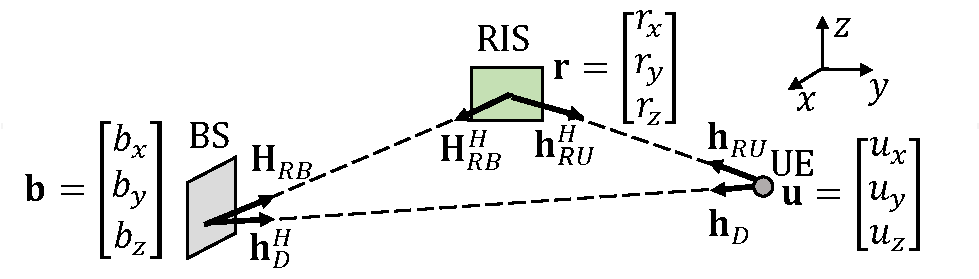
\includegraphics[width=.3569\textwidth, trim = {0cm .5cm 0cm 0cm}]{Figures/geometry_small_v2.pdf}
        \caption{\label{fig:system_model}
        Geometrical representation of the considered scenario, including the \gls{bs} position $\mb{b}$, the \gls{ris} position $\mb{r}$, and a \gls{ue} position $\mb{u}$.}
\end{figure}

We denote the \gls{ris} array response with the vector $\mb{a}_{\ssub{R}}(\mb{p}) \in \mathbb{C}^{N \times 1}$ with elements defined as the following
\begin{align}
    \{\mb{a}_{\ssub{R}}(\mb{p})\}^N_n \triangleq G(\mb{p}) e^{ -\jmath \frac{2 \pi }{\lambda} \left(\Vert \mb{p}-\mb{q}_n\Vert-\Vert \mb{p}-\mb{p}_{\text{ref}}\Vert \right)}, \label{eq:ris_response}
\end{align}
where $\mb{p} \in \mathbb{R}^3$ is the point of departure or arrival of the signal, $\lambda$ is the wavelength at the carrier frequency $f_0$, $\mb{q}_n=\mb{p}_n-\mb{p}_{\text{ref}}  \in \mathbb{R}^3$ is the offset between the absolute position $\mb{p}_n$ of the $n$-th \gls{ris} element and the arbitrary \gls{ris} reference point $\mb{p}_{\text{ref}} \in \mathbb{R}^3$, and $G(\mb{p})$ is the gain of the element 
in the direction of $\mb{p}$, which is 
$G(\mb{p}) = 1$ under the assumption of patch antenna elements. 

Importantly, Eq.~\eqref{eq:ris_response} accounts for the wavefront curvature at the \gls{ris} as it depends directly on the location $\mb{p}$, rather than on angles of arrival and departure only~\cite{abu2021near, rahal2021ris}. The \gls{bs} array response vector $\mb{a}_{\ssub{B}}(\bm{p}) \in \mathbb{C}^{M \times 1}$ is defined similarly.

Having defined the array steering vectors, we can now define the channels $\mb{H}_{\ssub{RB}}$, $\mb{h}_{\ssub{RU}}$, and $\mb{h}_{\ssub{D}}$ as follows
\begin{align}
    \{\{\mb{H}_{\ssub{RB}}\}^{M}_{m}\}^N_n &\triangleq \sqrt{\gamma(\mb{p}_n,\mb{p}_m)}\{\mb{a}_{\ssub{R}}(\mb{p}_m)\}_n\{\mb{a}^{\herm}_{\ssub{B}}(\mb{p}_n)\}_m, \label{eq:channel_bs_ris}\\
    \{\mb{h}_{\ssub{RU}}\}^N_n & \triangleq \sqrt{\gamma(\mb{p}_n,\mb{u})}\{\mb{a}_{\ssub{R}}(\mb{u})\}_n, \label{eq:channel_ris_ue}\\
    \{\mb{h}_{\ssub{D}}\}^M_m & \triangleq \sqrt{\gamma(\mb{p}_m,\mb{u})}\{\mb{a}_{\ssub{B}}(\mb{u})\}_m, \label{eq:channel_bs_ue}  
\end{align}
where $\gamma(\mb{x},\mb{y})$ is the path gain between two given locations $\mb{x}$, $\mb{y} \in \mathbb{R}^3$ and is defined as the following
\begin{align}
\gamma(\mb{x},\mb{y}) \triangleq \gamma_0 \left( \tfrac{d_0}{\|\mb{x} - \mb{y}\|} \right)^\beta,
\label{eq:path_gain}
\end{align}
where $\gamma_0$ is the channel power gain at a reference distance $d_0$ and $\beta$ is the pathloss exponent.

We consider a generic, non-ideal, channel estimation process that returns the estimation of $\hat{\mb{H}}_{\ssub{RB}}$, $\hat{\mb{h}}_{\ssub{RU}}$, and $\hat{\mb{h}}_{\ssub{D}}$ as \gls{csi}.

Moreover, we assume the presence of a phase selection agent that optimizes the \gls{ris} configuration based on the available \gls{csi}.
To ease the notation, we introduce an alternative but equivalent representation of $\mb{\Theta}$ with the definition of the following vector
\begin{align}
\boldsymbol{\uptheta} = \diag{ (\angle \mb{\Theta})} = \left[\theta_1, \theta_2, \dots, \theta_{\ssub{N}} \right]^\tran \in \{0,2\pi\}^{N \times 1}.
\end{align}
We denote the selected \gls{ris} configuration as $\bar{\boldsymbol{\uptheta}}$, and we describe the optimization process executed by the agent as 
\begin{align}
\bar{\boldsymbol{\uptheta}} =\angle \bar{\mb{\Theta}}&= g(\hat{\mb{H}}_{\ssub{RB}}, \hat{\mb{h}}_{\ssub{RU}}, \hat{\mb{h}}_{\ssub{D}}) = \underbrace{g(\mb{H}_{\ssub{RB}}, \mb{h}_{\ssub{RU}}, \mb{h}_{\ssub{D}})}_{\mb{\uptheta}^*} + \mb{e}_{\uptheta}, \label{eq:ris_configuration}
\end{align}
where $g(\cdot)$ is the \gls{ris} configuration optimization process, $\mb{\uptheta}^*$ is the optimal configuration obtained when perfect \gls{csi} is available, and $\mb{e}_{\uptheta}$ is the error introduced by the 
non-ideal channel estimation process.
Note that phase shift values can be either discrete or continuous, depending on the \gls{ris} design~\cite{fara2022prototype, rossanese2022designing}. We characterize $\bar{\boldsymbol{\uptheta}}$ in the continuous case, and face the discrete case later in this section.

In its most general form---as detailed in Section~\ref{sec:configuration_methods}---the configuring agent operates as a phase measurement device that extracts the phase of the \gls{csi}. 
Given the direct dependence of \newpage \gls{csi} quality on the \gls{snr},\footnote{\gls{csi} estimation techniques (as pilot signals) are impacted by \gls{snr}: higher \gls{snr} improves accuracy and vice versa (\cite{steven1993fundamentals}).}
we assume the spread of the error $\mb{e}_{\uptheta}$ to be inversely proportional to the \gls{snr}.

Furthermore, for the sake of tractability and without loss of generality, we assume phase measurements to be independent at each \gls{ris} element.
Hence, we model the error $\mb{e}_{\Theta}$ as a normal \gls{rv} with distribution  $\mb{e}_{\uptheta}\sim\mathcal{N}(\mb{0}_{\ssub{N}}, \sigma_{\theta}^2\mb{I}_{\ssub{N}})$, with $\sigma^2_\theta = \frac{1}{2\gamma}$, where $\gamma$ denotes the \gls{snr}.

Accordingly, $\bar{\boldsymbol{\uptheta}}$ is a normal \gls{rv} with distribution
\begin{align}
\bar{\boldsymbol{\uptheta}}\sim f_{\bar{\boldsymbol{\uptheta}}}(\bar{\boldsymbol{\uptheta}}) = \mathcal{N}(\boldsymbol{\uptheta}^*, \sigma^2_{\uptheta}\mb{I}_{\ssub{N}}). \label{eq:theta_distribution}
\end{align}

Section~\ref{sec:proof_of_gaussian_assumption} provides a formal demonstration of Eq.~\eqref{eq:theta_distribution}.

When considering an \gls{ris} hardware capable of discrete phase shifts, we assume the set of feasible configurations 
\begin{equation}
    \mathcal{Q} = \left\{\Delta m : m = 0,\dots, 2^{Q-1}, m \in \mathbb{N} \right\}, \label{eq:phase_quantization_set}
\end{equation}
 where $Q$ denotes the phase shifts quantization level, and $\Delta = \tfrac{2\pi}{2^Q}$. The total number of feasible configurations is $| \mathcal{Q} |=2^{Q}$. Phase shifts are set according to the quantization function $q: \mathbb{R} \rightarrow \mathcal{Q}$ defined as
\begin{equation}
q(x) = \Delta \left\lfloor \tfrac{x}{\Delta} + \tfrac{1}{2} \right\rfloor.
\end{equation}
The quantized \gls{ris} configuration is obtained as $\bar{\boldsymbol{\uptheta}}_{\ssub{Q}} = q(\bar{\boldsymbol{\uptheta}})$. Again, $\bar{\boldsymbol{\uptheta}}_{\ssub{Q}}$ is a \gls{rv}, which is distributed as the following 
\begin{align}
\bar{\boldsymbol{\uptheta}}_{\ssub{Q}}\sim f_{\bar{\boldsymbol{\uptheta}}_{\ssub{Q}}}(\bar{\boldsymbol{\uptheta}}_{\ssub{Q}}) =  \prod_{n=1}^{N} f_{\bar{\theta}_{\ssub{Q},n}}(\bar{\theta}_{\ssub{Q},n}), \label{eq:theta_distribution_quant}
\end{align}
with
\begin{align}
f_{\bar{\theta}_{\ssub{Q},n}}(\bar{\theta}_{\ssub{Q},n}) =  \sum_{m=0}^{2^{Q-1}} P\left(\bar{\theta}_{\ssub{Q},n}= \Delta m\right) 
\delta \left(\bar{\theta}_{\ssub{Q},n} - \tfrac{2\pi}{2^Q} m \right),\label{eq:theta_distribution_quant_el}
\end{align}
where $\delta(\cdot)$ is the delta function, and
\begin{equation}
P\left(\bar{\theta}_{\ssub{Q},n}= \Delta m\right) =  \int_{\Delta(m-0.5)}^{\Delta(m+0.5)} f_{\bar{\theta}_{n}}(\theta) d\theta
\end{equation}
is the probability of selecting $\bar{\theta}_{\ssub{Q},n}= \Delta m$.

\subsection{Optimizing RIS Configurations}
\label{sec:configuration_methods}

The \gls{ris} configuration process is generally complex, as it implies the joint optimization of the \gls{bs} precoder and the \gls{ris} configuration to maximize a given objective \glspl{kpi}, and is currently still an open problem~\cite{pan2022overview}. Hereafter, we summarize the main joint optimization strategies: $i$) \emph{Gradient optimization}: iterative adjustment of \gls{ris} configuration and \gls{bs} to optimize given metrics (e.g., \gls{snr}) in the direction of the gradient; $ii$) \emph{Alternating optimization}: optimization of each independent subproblem while keeping the other fixed~\cite{mursia2020risma,yu2020robust}; $iii$) \emph{\acrlong{ml}}: application of \gls{ml} agents to face \gls{ris} configuration problems~\cite{faisal2022machine,encinas2023unlocking}; $iv$) \emph{Coherent paths}: a practical approach that maximizes the gain of the reflected path while achieving constructive interference with the direct path~\cite{bjornson2019intelligent}.


\begin{figure}[t]
\centering

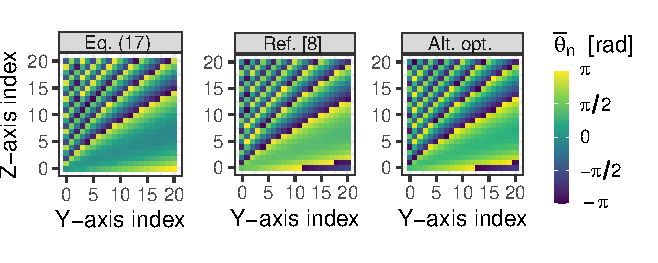
\includegraphics[width=1\linewidth, trim = {0cm 0.75cm 0cm 0cm}]{Figures/fig02.pdf}

\caption{\gls{ris} configurations from coherent paths optimization Eq.~\eqref{eq:coherent_solution}, optimization method from~\cite{bjornson2019intelligent} and alternate optimization algorithm from~\cite{mursia2020risma}.} \label{fig:coherent_vs_risma}
\end{figure}




Considering the coherent paths configuration solution, the \gls{ris} configuration process $g(\cdot)$ can be written in a closed form while still obtaining results comparable to more complex optimization procedures~\cite{albanese2022marisa}.
We anticipate that this optimization approach enables us to create offline ground-truth data that we use for training \name{}, as described in Section~\ref{sec:localization_method}.

\end{document}